%HW-design af Distancesensor
\section{Distancesensor} \label{sec:hw_design_distancesensor}

\begin{figure}[ht]
	\centering
	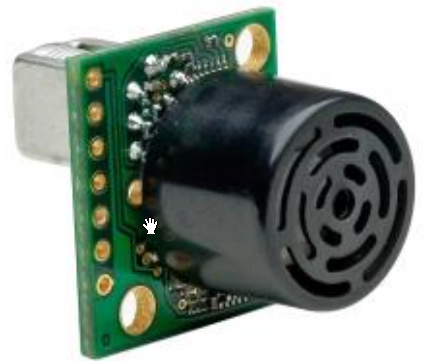
\includegraphics[scale=0.4]{../fig/billeder/distancesensor.png}
	\caption{Distancesensor MaxSonar1202}
	\label{fig:ds_pic}
\end{figure}

\newpage
Afstandssensorene leveres formonteret på print hvor benene fra IC'en er trukket til harwinpins som let kan tilgås. Til kommunikationen med sensoren benyttes \IIC via følgende 4 linjer: 

\begin{packed_item}
	\item pin 7: VCC: Forsyning
	\item pin 6: GND: Reference
	\item pin 5: SCL: Clock
	\item pin 4: SDA: Data
\end{packed_item}

\begin{figure}[ht]
	\centering
	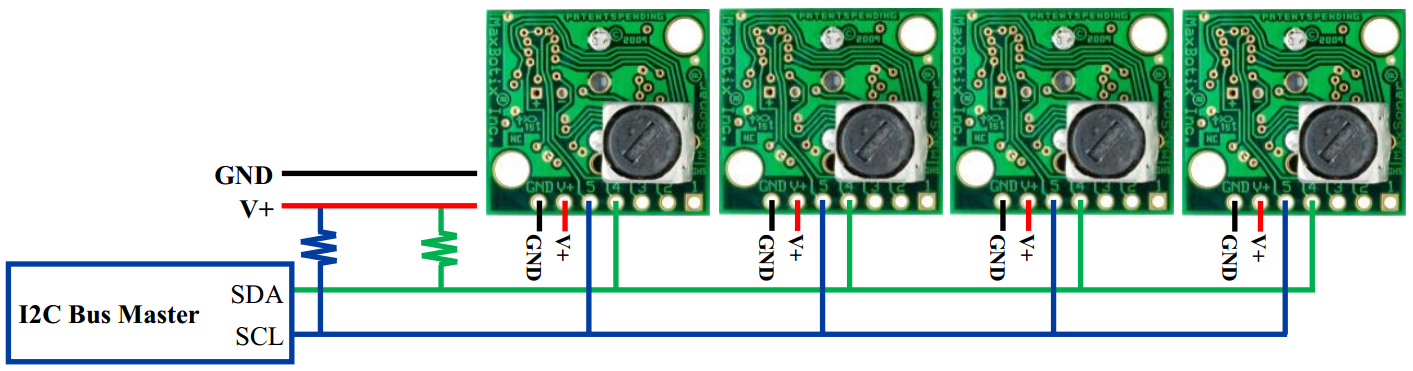
\includegraphics[scale=0.45]{../fig/billeder/distancesensor_multi.png}
	\caption{Distancesensor opsætning på AU2}
	\label{fig:ds_multi}
\end{figure}

Data kommunikeres på SDA-linjen med reference til GND, SCL styrer clocken. Så standard for \IIC kommunikation monteres der pull-up modstande på SDA og SCL linjerne da Bus Masteren ønsker at kunne trække disse lave.
Værdien for disse 2 modstande er sat til $4.7kHz$ da der arbejde med relative korte afstande. Printet ses på fig \ref{fig:i2c_print}. 

\begin{figure}[ht]
	\centering
	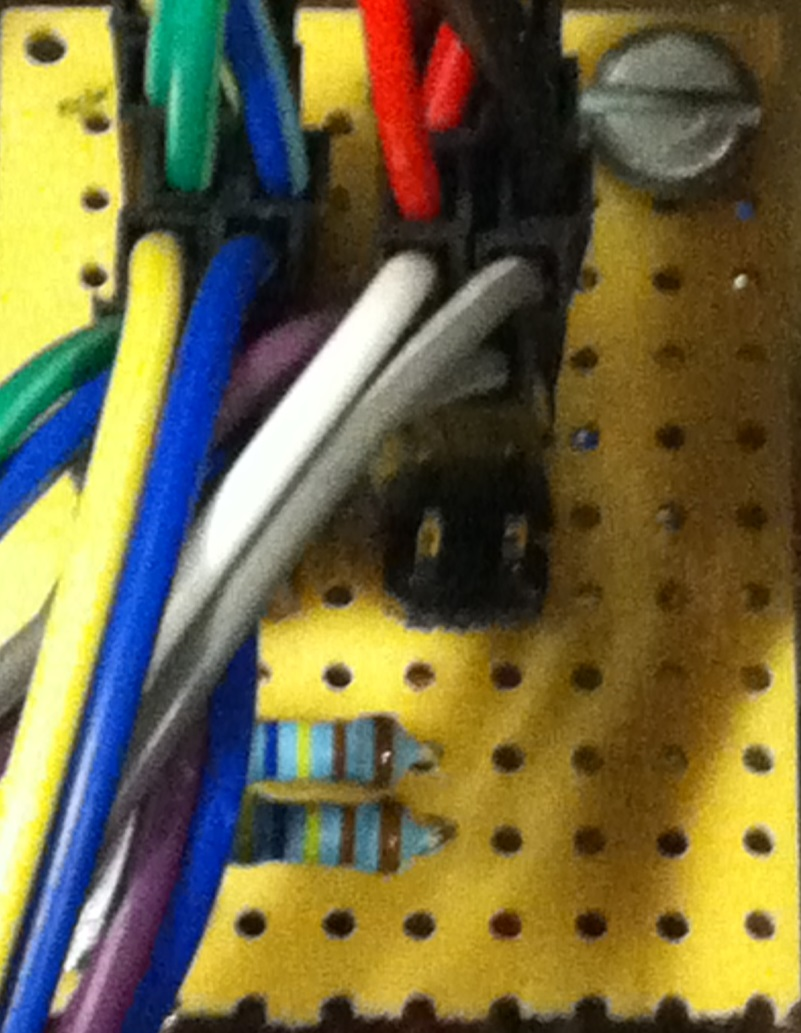
\includegraphics[scale=0.2]{../fig/billeder/I2C_print.jpg}
	\caption{Pull-up modstande til SDA go SCL linjerne til VCC}
	\label{fig:i2c_print}
\end{figure}

\newpage
Der benyttes de hardcodede default adresser til de 4 sensorer, disser er som følger: 

\begin{table}[ht]\centering
	\begin{tabular}{| l | l |} \hline
		\textbf{Sensor} 	& \textbf{Adresse}  \\\hline
		FL 					& \texttt{0x70} 	\\\hline
		FR 					& \texttt{0x71} 	\\\hline
		RL 					& \texttt{0x73} 	\\\hline
		RR 					& \texttt{0x76} 	\\\hline
	\end{tabular}
	\caption{Adresser på afstandssensorer}
	\label{table:adr_ds}
\end{table}


Til kommunikationen er valgt at bruge 7-bits adresser, og derudover følges protokollen på figur \ref{fig:ds_prtl}: 

\begin{figure}[ht]
	\centering
	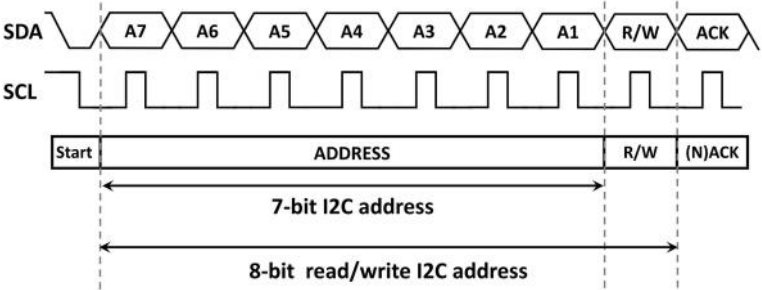
\includegraphics[scale=0.6]{../fig/billeder/distancesensor_protokol.png}
	\caption{\IIC protokol for distancesensor}
	\label{fig:ds_prtl}
\end{figure}

\texttt{write}-kommandoen fylder 1 byte + adresse, 2xACK samt start/stop-bit jf. protokollen på figur\ref{fig:ds_prtl}. 
\texttt{read}-kommandoen fylder 2 byte + adresse, 2xACK, NACK samt start/stop-bit jf. protokollen på figur\ref{fig:ds_prtl}

For verificering af dette henvises til moduletesten af PSoC'en-sensor kommunikation i afsnit \ref{sub:sw_impl_psoc_psoc} Software Implementering af PSoC på side \pageref{sub:sw_impl_psoc_psoc}

For at kunne benytte sensorerne skal der transmitteres en række kommandoer til de enkelte sensorer. Disse kommandoer skal overholde følgende fremgangsmåde:

\begin{enumerate}
  \item \textit{write}-mode-Kommando sendes til den given sensoradresse.
  \item Der kan nu skrives til sensoradressen
  \item \textit{read}-mode-Kommando sendes til den given sensoradresse.
  \item Der kan nu læses fra sensoradressen
\end{enumerate}

Alle \textit{write}- eller \textit{read}-kommandoer foregår altså som koblinger af 2 kommandoer, én hvor der sættes ''mode'' og til at foretage \texttt{read/write}. Det ses af figur \ref{fig:ds_prtl} at R/W-bitet har placering som A0.
Dette verificeres af følgende tabel over  \texttt{read/write}-kommandoer til/fra sensorerne: 

\begin{table}[ht]\centering
	\begin{tabular}{| l | l |} \hline
		\textbf{Kommando} & \textbf{Adresse} \\\hline
		FLwrite 	 & 0xE0 \\\hline
		FRwrite 	 & 0xE2 \\\hline
		RLwrite 	 & 0xE6 \\\hline
		RRwrite 	 & 0xEC \\\hline
		FLread  	 & 0xE1 \\\hline
		FRread  	 & 0xE4 \\\hline
		RLread  	 & 0xE7 \\\hline
		RRread  	 & 0xED \\\hline
		StartReading & 0x51	\\\hline
	\end{tabular}
	\caption{\textit{read/write}-kommandoer til afstandssensorer}
	\label{table:adr_ds_cmd}
\end{table}

Afsnit \ref{sub:sw_impl_psoc_psoc} Software Implementering af PSoC fra side \pageref{sub:sw_impl_psoc_psoc} beskriver detaljeret hvordan disse benyttes til at kommunikere med distancesensorerne.

 